\documentclass[a4paper]{article}
\usepackage[T1]{fontenc}
\usepackage[russian]{babel}
\usepackage[pdftex]{graphicx}
\usepackage[ruled,vlined]{algorithm2e}
\usepackage[utf8]{inputenc}
\usepackage{xcolor}
\usepackage{hyperref}
\usepackage{amsmath}
\usepackage{geometry}
\usepackage{float}
\usepackage{caption}
\usepackage{subcaption}
\DeclareGraphicsExtensions{.pdf,.png,.jpg}

\begin{document}

    \begin{titlepage}
        \Large
        \begin{center}
            Санкт-Петербургский \ Политехнический университет Петра Великого\\
            \vspace{10em}Отчет по лабораторной работе №1\\
            \vspace{2em}
            \textbf{Изучение характеристик распределений}
        \end{center}
        \vspace{6em}
        \hfill\parbox{10cm}{
            \hspace*{2cm}\hspace*{-4cm}Студент:\hfill Швачко Никита Андреевич\\
            \hspace*{2cm}\hspace*{-4cm}Преподаватель:\hfill Баженов Александр Николаевич\\
            \hspace*{2cm}\hspace*{-4cm}Группа:\hfill 5030102/20202
        }
        \vspace{\fill}
        \begin{center}
            Санкт-Петербург \ 2025
        \end{center}
    \end{titlepage}


    \section{Формулировка задания и его формализация}\label{sec:----2}
    Для 4 распределений:
    \\- Нормальное распределение $N(x, 0,1)$
    \\- Распределение Коши $C(x, 0,1)$
    \\- Распределение Пуассона $P(k, 10)$
    \\- Равномерное распределение $U(x,-\sqrt{3}, \sqrt{3})$
    \\1. Сгенерировать выборки размером 10,50 и 1000 элементов. Построить на одном рисунке гистограмму и график плотности распределения.
    \\2. Сгенерировать выборки размером 10,100 и 1000 элементов. Для каждой выборки вычислить следующие статистические характеристики положения данных:
    $\bar{x}, \operatorname{med} x, z_Q$. Повторить такие вычисления 1000 раз для каждой выборки и найти среднее характеристик положения и их квадратов:

    $$
    E(z)=\bar{z}
    $$


    \\  Вычислить оценку дисперсии по формуле:

    $$
    D(z)=\overline{z^2}-\bar{z}^2
    $$


    Представить полученные данные в виде таблиц.
    \\ Пояснение

    $$
    z_Q=\frac{z_{1 / 4}+z_{3 / 4}}{2}
    $$


    \section{Гистограммы и графики плотности распределений}\label{sec:----}
    \begin{figure}[H]
        \centering
        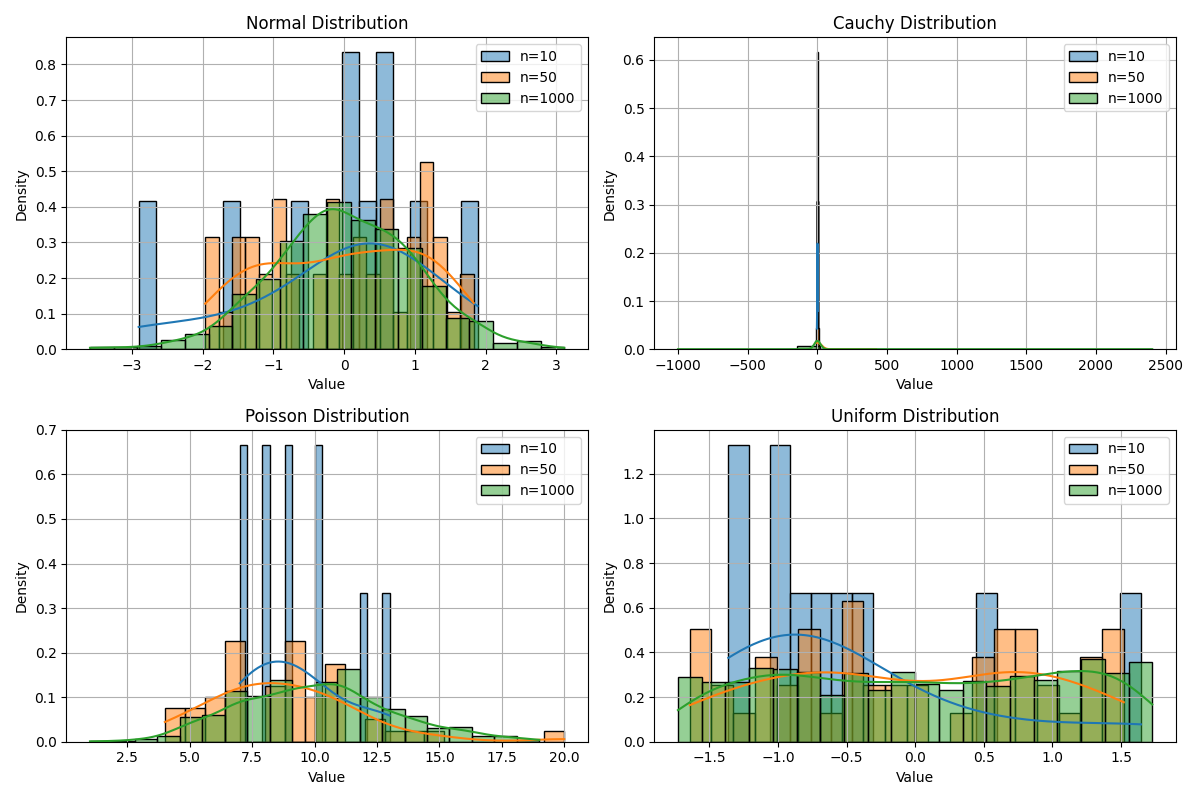
\includegraphics[width=1\textwidth]{histograms} % Вставить график
        \caption{Гистограммы и плотности распределений для выборок разного размера}\label{fig:figure}
    \end{figure}

    \newpage


    \section{Результаты вычислений статистических характеристик}\label{sec:---}
    \begin{table}[!htbp]
        \centering
        \caption{Средние значения характеристик положения и их дисперсии}

        \scalebox{0.8}{



            \begin{tabular}{|c|c|c|c|}
                \multicolumn{1}{|c|}{\textbf{Нормальное}} \\
                \hline
                \textbf{Выборка} & \textbf{Характеристика} & \textbf{E(z)} & \textbf{D(z)} \\
                \hline
                10               & $\bar{x}$               & -0            & 0.09          \\
                10               & $\operatorname{med} x$  & -0.01         & 0.13          \\
                10               & $z_Q$                   & -0            & 0.11          \\
                100              & $\bar{x}$               & 0             & 0.01          \\
                100              & $\operatorname{med} x$  & -0            & 0.02          \\
                100              & $z_Q$                   & -0            & 0.01          \\
                1000             & $\bar{x}$               & 0             & 0             \\
                1000             & $\operatorname{med} x$  & 0             & 0             \\
                1000             & $z_Q$                   & 0             & 0             \\
                \hline \\
                \multicolumn{1}{|c|}{\textbf{Коши}} \\
                \hline
                \textbf{Выборка} & \textbf{Характеристика} & \textbf{E(z)} & \textbf{D(z)} \\
                \hline
                10               & $\bar{x}$               & 0.75          & 283.65        \\
                10               & $\operatorname{med} x$  & 0.01          & 0.33          \\
                10               & $z_Q$                   & 0.01          & 0.86          \\
                100              & $\bar{x}$               & -0.46         & 205.23        \\
                100              & $\operatorname{med} x$  & 0             & 0.03          \\
                100              & $z_Q$                   & 0.01          & 0.05          \\
                1000             & $\bar{x}$               & -9.05         & 51968.84      \\
                1000             & $\operatorname{med} x$  & -0            & 0             \\
                1000             & $z_Q$                   & 0             & 0.01          \\
                \hline \\
                \multicolumn{1}{|c|}{\textbf{Пуассон}} \\
                \hline
                \textbf{Выборка} & \textbf{Характеристика} & \textbf{E(z)} & \textbf{D(z)} \\
                \hline
                10               & $\bar{x}$               & 10.04         & 1.06          \\
                10               & $\operatorname{med} x$  & 9.9           & 1.41          \\
                10               & $z_Q$                   & 9.98          & 1.19          \\
                100              & $\bar{x}$               & 10.01         & 0.09          \\
                100              & $\operatorname{med} x$  & 9.88          & 0.18          \\
                100              & $z_Q$                   & 9.93          & 0.14          \\
                1000             & $\bar{x}$               & 10            & 0.01          \\
                1000             & $\operatorname{med} x$  & 10            & 0             \\
                1000             & $z_Q$                   & 9.99          & 0             \\

                \hline \\
                \multicolumn{1}{|c|}{\textbf{Равномерное}} \\
                \hline
                \textbf{Выборка} & \textbf{Характеристика} & \textbf{E(z)} & \textbf{D(z)} \\
                \hline
                10               & $\bar{x}$               & 0.01          & 0.1           \\
                10               & $\operatorname{med} x$  & 0.01          & 0.22          \\
                10               & $z_Q$                   & 0.01          & 0.14          \\
                100              & $\bar{x}$               & -0            & 0.01          \\
                100              & $\operatorname{med} x$  & -0.01         & 0.03          \\
                100              & $z_Q$                   & -0            & 0.01          \\
                1000             & $\bar{x}$               & 0             & 0             \\
                1000             & $\operatorname{med} x$  & 0             & 0             \\
                1000             & $z_Q$                   & 0             & 0             \\
                \hline
            \end{tabular}
        }
        \label{tab:table}
    \end{table}


    \section{Выводы}\label{sec:}
    \begin{itemize}
        \item При увеличении размера выборки характеристики положения стабилизируются.
        \item Среднее значение $\bar{x}$ для распределения Коши не является надежным из-за сильных выбросов.
        \item Медиана и квартильный средний $z_Q$ показывают меньшую изменчивость в выборках с выбросами.
        \item Пуассоновское распределение при больших $n$ приближается к нормальному.
        \item Равномерное распределение демонстрирует низкую изменчивость статистик.
    \end{itemize}


\end{document}
